% General stuff
\documentclass[french]{article}
\author{André Madeira Cortes}
\date{2019-2020}
\usepackage{geometry}
\geometry{a4paper, left=30mm, right=35mm, top=30mm, bottom=25mm,}
\usepackage{float}

% Global packages
\usepackage[utf8]{inputenc}
\usepackage[T1]{fontenc}
\usepackage{babel, graphicx, blindtext, scrextend, hyperref, tikz, amsmath}

% Footnotes
\usepackage[side]{footmisc}
\renewcommand{\thefootnote}{\roman{footnote}}

% Epigraphs
\usepackage{epigraph}
\setlength\epigraphwidth{1\textwidth}
\setlength\epigraphrule{0pt}
\setlength\beforeepigraphskip{1\baselineskip}
\setlength\afterepigraphskip{2\baselineskip}
\renewcommand*{\textflush}{flushright}
\renewcommand*{\epigraphsize}{\normalsize\itshape}

% Lecture command definition
\usepackage{xifthen}
\def\testdateparts#1{\dateparts#1\relax}
\def\dateparts#1 #2 #3 #4 #5\relax{
    \marginpar{\small\textsf{\mbox{#1 #2 #3 #5}}}
}

\def\@lecture{}%
\newcommand{\lecture}[2]{
    \def\@lecture{\textsf{Cours #1} - \textsf{\mbox{#2}}}%
}

% Fancy headers
\usepackage{fancyhdr}
\pagestyle{fancy}

\fancyhead[R]{\@lecture} % Right odd,  Left even
\fancyfoot[C]{}          % Center
\rfoot{\thepage}
\renewcommand{\footrulewidth}{1pt}
\makeatother

\graphicspath{{images/}}

% Extra packages
\usepackage{eurosym}
% Tikz packages
\usepackage{tikz, tikz-qtree}
\usetikzlibrary{positioning}

\title{STIC-B425 - Ingénierie linguistique\\Notes de cours}

\begin{document}

\maketitle
\setcounter{tocdepth}{2}
\tableofcontents
\newpage

\lecture{1}{mardi 04 février 2020}
\vspace{-1.2cm}

\section{Introduction au cours}

Qu'est-ce que l'ingénierie linguistique? Le nom de ce cours est ancien, aujourd'hui on dirait plutôt
"Introduction au Traitement Automatique des Langues (TAL)". On garde cet ancien nom car il est
intéressant (il mets en évidence qu'il s'agit d'un mix entre sciences "dures" et sciences "sociales"). \\

Il s'agit d'une discipline en constante évolution et hybride. Historiquement, deux disciplines dissociées et
ayant des chercheurs distincts existaient: d'un coté des linguistes s’interrogeant sur ce que l'informatique
pourrait apporter à leur discipline (linguistique informatique), et de l'autre des informaticiens et ingénieurs
curieux d'appliquer leurs modèles mathématiques dans l'étude de la linguistique (traitement automatique des langues).
À présent, les deux disciplines sont communes. \\

\textbf{Applications possibles de la discipline:}\\

\begin{minipage}[t]{0.5\textwidth}
\begin{itemize}
\item Correction orthographique/grammaticale
\item Traduction automatique/assistée
\item Reconnaissance et synthèse vocale
\end{itemize}
\end{minipage}
\begin{minipage}[t]{0.5\textwidth}
\begin{itemize}
\item Extraction d'informations
\item Analyse de sentiments
\item Question answering
\end{itemize}
\end{minipage}

\subsection{Niveaux linguistiques}

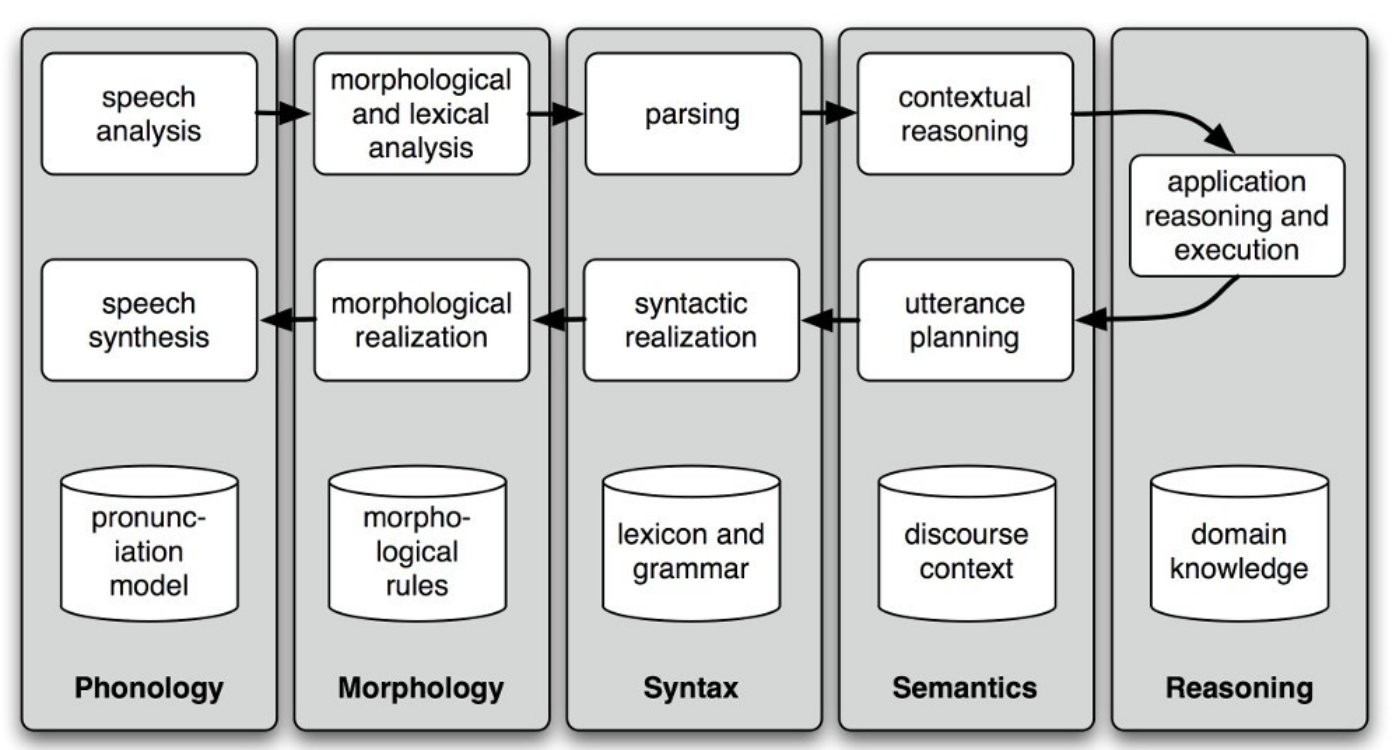
\includegraphics[scale=0.3]{lec1img1}\\ \\

Dans ce cours on étudie les nombreux niveaux linguistiques existants et les challenges qu'ils apportent au niveau
de l'ingénierie linguistique, car le langage humain est ambigu à tous les niveaux.\\

\begin{itemize}
    \item \textbf{Phonétique / Phonologie}: Hors scope du cours. Reconnaissance de mots depuis un signal audio et
    génération d'un signal audio à partir de mots. Prononciation, réalisation acoustique, etc.
    \item \textbf{Morphologie}: Reconnaissance des variations de forme des mots individuels (pluriel, conjugaison,...).
    \item \textbf{Lexique}: Qu'est-ce qu'un mot? Il faut savoir comment découper une phrase en mots pour la traiter par la suite.
    \item \textbf{Syntaxe}: Reconnaissance de l'ordre des mots et de l'organisation interne d'une phrase structurée.
    \item \textbf{Sémantique}: Reconnaissance du sens intrinsèque des mots (sémantique lexicale) ainsi que de la manière dont
    ils s'influencent mutuellement (sémantique compositionnelle).
    \item \textbf{Pragmatique}: Brièvement discuté lors du cours, mais hors scope du cours. Reconnaissance de l'intention du
    locuteur de la manière appropriée d'y répondre en fonction du contexte.
\end{itemize}

\subsection{Challenges affrontés}

\textbf{Ambigüités possibles:}

\begin{itemize}
    \item \textbf{Ambigüité phonétique}: Homophonie
    \item \textbf{Ambigüité morpho-lexicale}: Homographie
    \item \textbf{Ambigüité syntaxique}
    \item \textbf{Ambigüité sémantique}
    \item \textbf{Sémantique}: Hors contexte, certaines phrases peuvent être lues de façons différentes
    \item \textbf{Ambigüité pragmatique}: Ironie, par exemple
    \item \textbf{Ambigüité multilingue}
\end{itemize}

\noindent\textbf{Contraintes supplémentaires:}

\begin{itemize}
    \item \textbf{Précision}: Reproduire la compétence linguistique des êtres humains à l'aide de modèles
    formalisant notre compréhension
    \item \textbf{Rappel}: Une bonne couverture de la langue traitée requiert des ressources
    linguistiques (lexiques, grammaires,...) suffisamment fournies
    \item \textbf{Performance}: Un traitement rapide implique de limiter la complexité des modèles linguistiques
\end{itemize}

\subsection{Un peu d'histoire}

(TO DO)

\newpage
\lecture{2}{vendredi 07 février 2020}
\vspace{-1.2cm}

\section{Introduction à la Traduction Automatique (TA)}

\epigraph{(…) the attempt to automate all, or part of the process\\ of translating from one human language to another.}{\textit{Arnold, 1993}}

Définition de Traduction Automatique: Automatisation du processus de traduction d'une $Phrase_{source} \rightarrow Phrase_{cible}$.
Il s'agit d'un domaine en constante évolution. Il envisage l'exercice de traduction comme s'il s'agissait d'un processus de décodage. \\

\noindent Il existe 3 types de traduction automatique:

\begin{enumerate}
    \item \textbf{Assimilation} Rompre la barrière des langues. Comprendre à minima le contenu d'un texte.
    On parle souvent de "gisting". Il y a de nombreuses applications: communication interne, blogs, journaux,
    sites web, documentation, littérature, etc. Il existe peu d'évaluation quantitative de ce genre de traduction.
    De toute façon, comment évaluer une telle traduction? Son but n'est pas d'être optimale, mais juste de couvrir
    au minimum la compréhension du texte source. Autre problème: de nombreux services de traduction online stockent
    les textes source, il y a donc un risque de problèmes de protection des données.
    \item \textbf{Communication} TA pour la communication orale (interprétation). Deux technologies centrales: la synthèse vocale et la TA.
    \item \textbf{Dissémination} TA du traducteur. Son but est de publier un texte dans une autre langue.
    La qualité doit être égale à la TH (traduction humaine), et il y a deux conditions pour que ce soit le cas
    \begin{enumerate}
        \item \textbf{Domaine limité} On essaye d'avoir une TEAHQ (Traduction Entièrement Automatique et de Haute Qualité) / FAHQT (Fully Automatic High Quality Translation).
        Ceci est impossible si on essaye de traduire dans un scope de langage énorme.
        Donc on essaye de focaliser les efforts sur un sous-langage (e.g. un traducteur spécialisé dans le domaine de la météo).
        \item \textbf{Intervention humaine} Un humain (traducteur ou réviseur) intervient dans le processus de traduction,
        de deux façons possibles: pré-édition (simplification du texte, éviter les phrases longues et les longs groupes nominaux, etc)
        et post-édition (PE). De nouveaux métiers se créent (sujet complexe car on dit également que d'autres métiers se perdent).
    \end{enumerate}
\end{enumerate}

\noindent Dans les prochains chapitres on analysera les trois types de systèmes de traduction automatique:

\begin{enumerate}
    \item \textbf{Systèmes linguistiques} Rule-based machine translation (RBMT) \footnote{\hyperref[sec:RBMT]{Chapitre 3}}
    \item \textbf{Systèmes fondés sur les corpus (data-driven)} \footnote{\hyperref[sec:corpus]{Chapitre 4}}
    \begin{enumerate}
        \item Statistical machine translation (SMT)
        \item Neuronal machine translation (NMT) \\
    \end{enumerate}
\end{enumerate}

\noindent\textbf{Post-édition VS Traduction Humaine}
\begin{enumerate}
    \item Rentable, 20\% à 40\% de gain de productivité selon les études (e.g. Plitt \& Masselot 2010, Green 2013)
    \item Ne conduit pas nécessairement à plus d'erreurs ou des textes de moins bonne qualité
    \item "Posteditese" (e.g. Toral 2019, Kubler 2019) (TODO: Add definition here)
\end{enumerate}

\noindent\textbf{Nouvelles applications de la TA\\}

\begin{minipage}[t]{0.5\textwidth}
\begin{itemize}
\item Sous-titrage
\item TA d'images
\item TA vers des langues simplifiées \\(e.g. Simple Wikipedia)\\
\end{itemize}
\end{minipage}
\begin{minipage}[t]{0.5\textwidth}
\begin{itemize}
\item TA vers des pictogrammes
\item TA vers la langue des signes
\end{itemize}
\end{minipage}

\noindent\textbf{Problèmes posés par la TA}

\begin{enumerate}
    \item \textbf{Ambigüité}
    \begin{enumerate}
        \item Lexicale
        \item Structurale
    \end{enumerate}
    \item \textbf{Divergences}
    \begin{enumerate}
        \item Lexicales (décalages)
        \item Structurales
    \end{enumerate}
    \item \textbf{De nombreuses traductions possibles}
        Comment choisir la meilleure (ou la seule correcte)?
\end{enumerate}

\noindent\textbf{Divergences structurales\\}

(TODO)

- Typologiques
    - Ordre des mots (e.g. SVO en FR, SOV en Japonais et VSO en Arabe)
    - Pronoms
- Idiosyncratiques (propres à une langue)
- Générales à la syntaxe d'une langue
- Déclenchées par un mot particulier

Du plus facile au plus compliqué à résoudre (Vandooren 1993)
- Catégorielle (e.g. nom vers adjectif)
- Syntagmatique
- Lexicale
- De densité lexicale
- Thématique
- Prédicative

Statistiques des divergences (Dorr 2002)
- Part of Speech (98\%)
- Phrase/Light verb (83\%)
- Structural (35\%)
- Heads swap (8\%)
- Arguments swap (6\%)

(END OF TODO)

\newpage

\section{Les systèmes linguistiques (RBMT)}
\label{sec:RBMT}

Les premiers systèmes de TA commerciaux et sur internet (BabelFish, Altavista, etc).
Ils étaient les seuls à être développés jusqu'en 2006 (avant l'apparition de SMT et NMT, voir chapitre suivant).

À l'époque ils étaient les seuls à faire de la TEAHQ (à mettre en perspective, la qualité n'est plus considérée aussi bonne quand on la compare aux résultats actuels).

Beaucoup de différences entre ces systèmes, mais quelques points communs:

\begin{enumerate}
    \item \textbf{Analyse linguistique} pour extraire le sens de la phrase
    ("natural language understanding")
    \begin{enumerate}
        \item Pipeline linguistique (on passe par différents niveaux: lexical,
        syntaxique, sémantique, pragmatique/extralinguistique)
    \end{enumerate}
    \item \textbf{Transfert}
    \item \textbf{Géneration} de la langue cible
\end{enumerate}

\subsection{Systèmes directs/minimalistes}

Les plus simples. Fonctionnent en deux étapes:

\begin{enumerate}
    \item \textbf{Compréhension minimale (lexicale)}
    \begin{enumerate}
        \item Segmentation en mots
        \item Tagging de catégorie grammaticale de chaque mot
    \end{enumerate}
    \item \textbf{Traduction} mot à mot avec un dictionnaire bilingue
\end{enumerate}

\textbf{Dictionnaire}

La ressource principale des systèmes directs (pas de grammaires).

Il contient toutes les informations nécessaires pour la compréhension et la traduction,
c'est à dire au minimum: le mot/expression source/cible, les informations lexicales monolingues sur le mot/expression source/cible et les informations bilingues.\\

\textbf{Informations bilingues}

\begin{enumerate}
    \item Traduction mots/expressions
    \item Tests (transfer conditions)
    \begin{itemize}
        \item Permettent de choisir la bonne traduction s'il y en a plusieurs.
        \item Devraient porter sur tous les niveaux linguistiques (lexical, synt, sem et pragmatique).
        \item e.g. : grow (élever, cultiver ou grandir?)
    \end{itemize}
    \item Actions
\end{enumerate}

\textbf{Types de tests}

\begin{itemize}
    \item Test sur les informations morphologiques (e.g. singulier vs pluriel)
    \item Test sur la syntaxe (rection) (e.g. traduction d'un verbe dépendant de
    l'objet auquel il s'applique)
    \item Test sur le type sémantique (sens) (e.g. traduction d'un verbe dépendant
    du type de sujet, humain ou animal)
    \item Test sur le domaine (e.g. le mot "bug" en informatique ou en biologie)
    \item Test sur les propriétés encyclopédiques (ontologie) (e.g. traductions
    entières de bouts de phrases stockées)\\
\end{itemize}

Dans les systèmes directs, les tests portent uniquement sur le niveau lexical:
nombre, genre, mots dans contexte.

Exemple: SystranNet (2018)

to grow (context: child, etc.) = grandir

to grow (context: chicken, etc.) = élever

to grow (context: corn, salad, etc.) = cultiver \\

\textbf{Actions}

Permettent de traiter les divergences, c'est-à-dire de changer la syntaxe sous
certaines conditions.

(TODO)
---
en TROIS étapes??

Compréhension
    Problèmes:
        - Analyse morphologique et résolution des homographes ca
Traduction
    Problèmes:
        - Tests/actions limités
        - 1 dictionnaire par paire de langues
Génération
    Problèmes:
        - Architecture de type "transformateur"
        - Pas de connaissances grammaticales de la langue cible, comme dans les systèmes indirects

---
Ne peut donner des résultats exploitables que si sous-langage et dictionnaire bien spécialisé

(END TODO)

\subsection{Systèmes indirects/maximalistes}

Tandis que les systèmes directs focalisaient le moins possible sur le niveau de
la compréhension (minimalistes), les systèmes indirects eux le font au plus possible.

Ils sont les seuls systèmes linguistiques à faire de la TEAHQ.\\

\textbf{Caractéristiques}

\begin{enumerate}
    \item Ne restent pas au niveau lexical. Font au moins une analyse syntaxique complète, avec une grammaire, et représentent ainsi le sens de la phrase à traduire
    \item Ne mettent pas en relation directe des mots, mais mettent en correspondance des représentations
\end{enumerate}

\textbf{Avantages}

\begin{enumerate}
    \item Représentent l’ambigüité structurale
    \item Évitent les erreurs de désambigüisation lexicale
\end{enumerate}

Systèmes de TA indirects
    - Par transfert
    - Par interlangue

Théories de la traduction circa '90
    - Deverbalisation du sens
    - Production

\vspace{1cm}

\textbf{Triangle de Vauquois}

\resizebox{0.85\textwidth}{!}{
    

\tikzset{every picture/.style={line width=0.75pt}} %set default line width to 0.75pt

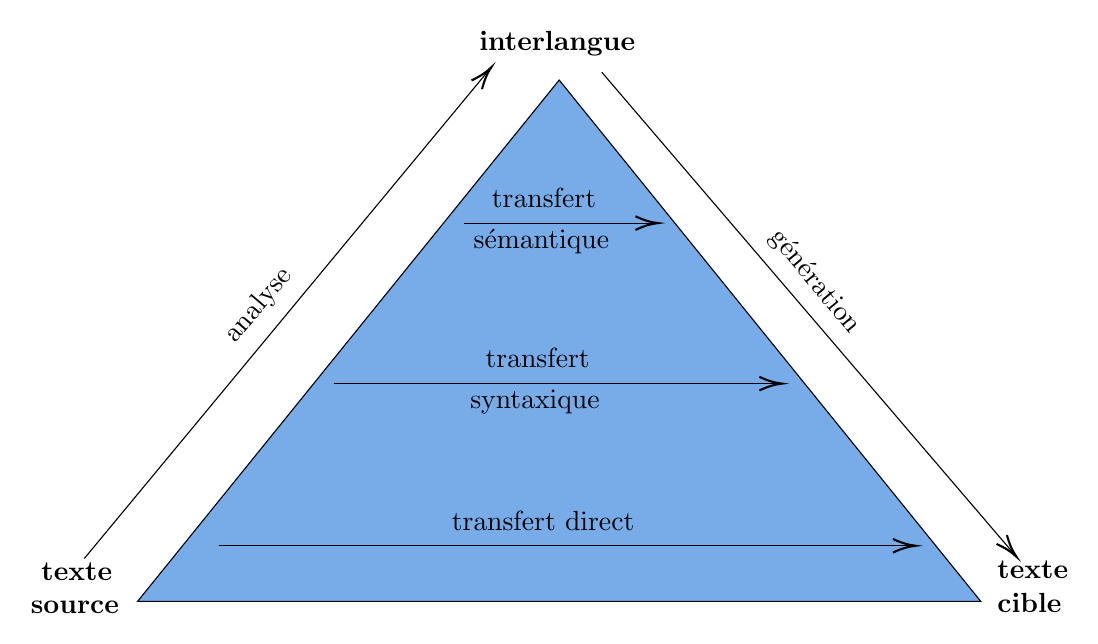
\begin{tikzpicture}[x=0.75pt,y=0.75pt,yscale=-1,xscale=1]
%uncomment if require: \path (0,777); %set diagram left start at 0, and has height of 777

%Shape: Triangle [id:dp37993567465978106]
\draw  [fill={rgb, 255:red, 74; green, 144; blue, 226 }  ,fill opacity=0.75 ] (297.6,38.51) -- (500.73,289.68) -- (94.48,289.68) -- cycle ;
%Straight Lines [id:da3821484196531547]
\draw    (133.92,262.88) -- (467.33,262.88) ;
\draw [shift={(469.33,262.88)}, rotate = 180] [color={rgb, 255:red, 0; green, 0; blue, 0 }  ][line width=0.75]    (10.93,-3.29) .. controls (6.95,-1.4) and (3.31,-0.3) .. (0,0) .. controls (3.31,0.3) and (6.95,1.4) .. (10.93,3.29)   ;
%Straight Lines [id:da35117354484946606]
\draw    (189.05,184.77) -- (403.01,184.77) ;
\draw [shift={(405.01,184.77)}, rotate = 180] [color={rgb, 255:red, 0; green, 0; blue, 0 }  ][line width=0.75]    (10.93,-3.29) .. controls (6.95,-1.4) and (3.31,-0.3) .. (0,0) .. controls (3.31,0.3) and (6.95,1.4) .. (10.93,3.29)   ;
%Straight Lines [id:da19792780780087094]
\draw    (251.85,107.43) -- (343.28,107.43) ;
\draw [shift={(345.28,107.43)}, rotate = 180] [color={rgb, 255:red, 0; green, 0; blue, 0 }  ][line width=0.75]    (10.93,-3.29) .. controls (6.95,-1.4) and (3.31,-0.3) .. (0,0) .. controls (3.31,0.3) and (6.95,1.4) .. (10.93,3.29)   ;
%Straight Lines [id:da14845116336104136]
\draw    (68.83,269.01) -- (263.59,33.92) ;
\draw [shift={(264.87,32.38)}, rotate = 489.64] [color={rgb, 255:red, 0; green, 0; blue, 0 }  ][line width=0.75]    (10.93,-3.29) .. controls (6.95,-1.4) and (3.31,-0.3) .. (0,0) .. controls (3.31,0.3) and (6.95,1.4) .. (10.93,3.29)   ;
%Straight Lines [id:da355143642126483]
\draw    (318.12,34.73) -- (516.63,266.67) ;
\draw [shift={(517.93,268.19)}, rotate = 229.44] [color={rgb, 255:red, 0; green, 0; blue, 0 }  ][line width=0.75]    (10.93,-3.29) .. controls (6.95,-1.4) and (3.31,-0.3) .. (0,0) .. controls (3.31,0.3) and (6.95,1.4) .. (10.93,3.29)   ;

% Text Node
\draw (257.83,13.54) node [anchor=north west][inner sep=0.75pt]   [align=left] {\textbf{{interlangue}}};
% Text Node
\draw (507.5,269.15) node [anchor=north west][inner sep=0.75pt]   [align=left] {\textbf{texte}\\\textbf{cible}};
% Text Node
\draw (41.79,269.92) node [anchor=north west][inner sep=0.75pt]   [align=left] {\textbf{ texte}\\\textbf{source}};
% Text Node
\draw (244.58,244.81) node [anchor=north west][inner sep=0.75pt]   [align=left] {transfert direct};
% Text Node
\draw (260.87,166.7) node [anchor=north west][inner sep=0.75pt]   [align=left] {transfert};
% Text Node
\draw (253.52,186.61) node [anchor=north west][inner sep=0.75pt]   [align=left] {syntaxique};
% Text Node
\draw (263.94,89.35) node [anchor=north west][inner sep=0.75pt]   [align=left] {transfert};
% Text Node
\draw (255.12,109.26) node [anchor=north west][inner sep=0.75pt]   [align=left] {sémantique};
% Text Node
\draw (132.51,159.58) node [anchor=north west][inner sep=0.75pt]  [rotate=-310.5] [align=left] {analyse};
% Text Node
\draw (406.04,106.74) node [anchor=north west][inner sep=0.75pt]  [rotate=-50.3] [align=left] {génération};


\end{tikzpicture}

}

\vspace{1cm}

Axe vertical: profondeur d'analyse, niveau d'analyse syntaxique
    e.g. directs on reste au niveau lexical, transfert au moins syntaxique, interlingue on va jusqu'au niveau sémantique

Axe horizontal: quantité de connaissance contrastive qu'il faut pour passer d'une langue à l'autre

Systèmes par transfert:

    - Module d'analyse: syntaxique et spécifique à la langue (par définition)
    - Module de transfert: règles de transfert
    - Génération: Représentation syntaxique cible -> texte cible

Types de règles de transfert:

    - Lexicales: équivalences entre les mots
    - Structurales: liens entre les éléments structuraux (e.g. verb --> verbe, subject -> sujet)
    - Semi-lexicales: permettent de changer la syntaxe de la phrase via des tests et actions

Avantages:

Systèmes par interlangue

Problèmes:
    - Concepts: définir l'ensemble des concepts et choisir le bon contexte. Ceci oblige à faire des distinctions qui ne sont pas nécessaires pour toutes les paires de langues. E.g. espagnol: différence entre le mot pour poisson vivant et poisson mort.
    - Granularité de la représentation:

Dionysus:
    Facteurs pragmatiques:
        Formalité: formel ou pas
        Simplicité: simple ou pas
        Force
        Couleur
        Respect
    Relations entre les phrases
        Domaine (cause, motivation), textuelle (conclusion, reformulation), temporelle
    Attitude
        emphase, croyance, négative, positive
    Intention
        question, requête


Différences transfert vs interlangue
    Types de représentation
        Transfert: spécifique à la langue
    Connaissances contrastives
    Type de traduction
        Transfert: littérale, on préserve la syntaxe
        Interlangue: par paraphrase, on va vers le sens et on génère avec le sens de la phrase

Exemples:
    Première par transfert
    Deuxième par interlangue

Exemples d'interlangue:
    UNL (ONU)
    Ontologie -> concepts communs à toutes les langues

    Esperanto
    Distributed Language Translation


Contexte positif pour l'interlangue
    - Sous dommaine, si possible technique
        - Travail humain énorme
    - Contexte multilingue
        - un seul système, au lieu d'un système par chaque paire de langues
    - Langues très différentes
        - e.g. Japonais, le transfert ne fonctionne pas vu la différence énorme au niveau de la grammaire

Systèmes linguistiques résumé
    Très ambitieux
    Hypothèses:
        - Bcp de régularités entre les langues: faux
        - Peu d'exceptions: faux
        - Règles peuvent être définies par des experts
    Problèmes:
        - Robustesse: les langues ne sont pas si régulières
        - Chers et lents à développer
        - Statiques: figés dans le temps, n'apprennent pas via de nouveaux corpus.

\newpage
\lecture{3}{samedi 08 février 2020}
\vspace{-1.2cm}

\section{Systèmes fondés sur les corpus}
\label{sec:corpus}

Apprennent les connaissances à partir des corpus ("data-driven")

- Connaissances probabilistes
- SMT (statistiques)
    - Restent au niveau de mots
    - Apprennent des mots + associations entre mots
- NMT (neuronaux)
    - Représentent la sémantique du mot


Idée corpus vs règles
Pionniers:

Nagao (1984)
    Les traducteurs ne ferraient pas une traduction complète de la phrase source. Il propose la base de l'approche statistique. Décomposer la phrase source en segments, puis on traduit les différents segments. À la phase on recompose ces différents segments pour reconstruire la phrase.
Isabelle (1992)
    Les traductions existantes (corpus) contiennent plus de solutions à des problèmes de traduction que n'importe quelle autre ressource (e.g. des dictionnaires).


\subsection{SMT}

Historique:
    - Première technologie envisagée (c.f Weaver)
    - 1990: premier article à IBM (Brown)
    - 2006: Google lance le premier système SMT, Google Translate
    - 2007: Plateforme open-source "Moses" (EuroMatrix) pour développer des systèmes SMT (sous la direction de Koehn)
    - État de l'art jusqu'en 2016

2 générations de SMT
    - TA statistique par mots (word-based machine translation)
    - TA statistique par segments (phrase-based machine translation)

Objectif SMT
    -Trouver pour une phrase Source la phrase Target qui a la plus grande probabilité d'être la traduction de la phrase S

``The target turn''
    - Choisir la bonne solution en Langue Cible, plutôt que d'analyser la Langue Source

Fonctionnement SMT
    Entrainement
        Corpus Parallèles (bilingues) et Corpus monolingue de la langue cible
        Analyses statistiques
        On extrait les mots et les associations bilingues/monolingues qui se trouvent dans les corpus, avec leurs fréquences
        On mets tout ça dans des modèles de traduction/langage.
        Modèle de traduction: fidélité. Regarde si phrase cible est bonne traduction à partir des mots source.
        Modèle de langage: Regarde si la phrase cible est fluide. ``qui se lit bien en langue cible''
        On décompose le problème de traduction en deux tâches.
    Décodage
        fidélité X fluidité
        On trouve le meilleur score qui soit un compromis entre ces deux concepts.
        Il y a plusieurs modèles statistiques: certains mettent le même poids aux deux modèles, d'autres apporteront plus de poids à l'un d'eux.

Traduction (noisy channel model)
    Problème de décision
        Trouver la meilleure phrase parmi toutes les phrase possibles
        $Translation = Argmax_T P(T) P(S|T)$
        P(T) provient du modèle de langue
        P(S|T) provient du modèle de traduction
        On veut trouver P(T|S)

Modèle de langue
    Objectif: déterminer le score de fluidité de la langue cible P(T)

    N-grammes - séquences de N mots
        Unigramme, bigramme, trigramme
        Il faut trouver un compromis: N-gramme trop petit -> pas hyper représentatif de la langue; N-gramme trop grand -> la probabilité de trouver cette chaine dans le corpus est plus petite
        On dépasse rarement 6-gramme dans l'état actuel des choses.

    Entrainement
        Prend le corpus monolingue
        Extrait tous les N-grammes
        Calcule leur probabilité dans le corpus monolingue, c’est-à-dire leur fréquence dans le corpus

    N-grammes lissés
    True casing

Modèle de traduction
    Objectif: déterminer quelle est la traduction la plus fidèle
    Intuitivement: on regarde dans le corpus bilingue dans quelle mesure chaque mot/segment de T est la traduction des mots/segments de la langue S


(.... see slides)

Limites
    - Gros corpus nécessaires: monolingues et bilingues
    - Traduisent par segments: Contexte limité à 5-6 mots
    - Fautes non locales
    - Ne généralisent pas : si le mot est absent du corpus, il n’est pas traduit

Statistiques VS Linguistiques
    - Raisons économiques: moins couteux (outils «open source»)
    - Pas de ressources linguistiques nécessaires (dictionnaires, grammaires, etc.): seule solution pour les langues peu dotées
    - Meilleure fluidité que les systèmes linguistiques
    - Se marie bien avec les mémoires de traduction. Pourquoi ?

Inconvénients
    - Nécessite des corpus représentatifs et assez grands
    - Moins précis (moins de fidélité)
        - Risque de contresens plus important, même si la phrase semble naturelle
    - Difficile à améliorer/modifier de manière transparente
    - Fonctionne mieux pour des langues proches, sans trop de divergences
    - Erreurs pas toujours systématiques -> plus difficile à post-éditer
        - e.g. Ma femme a sauté un repas vs Ma belle femme a sauté un repas
    - Nécessite pas mal de ressources informatiques pour les estimer/stocker les modèles

Références:
    Statistical Machine Translation by Koehn
    Statistical Machine Translation: A guide for linguists and translators (2011)

\newpage
\lecture{4}{vendredi 21 février 2020}
\vspace{-1.2cm}

\subsection{NMT}

Dernière génération des systèmes de TA \\

\begin{itemize}
    \item 2016: GT lance le 1er système neuronal sur le web
    \item 2017: DeepL
    \item Aujourd'hui: presque tous les systèmes sur internet sont neuronaux sauf Yandex (hybride SMT/NMT) et Apertium (RBMT)
    \item 2019: Reverso (Reverso Corporate)\\
\end{itemize}

Plateforme open source: OpenNMT

Plateforme commerciale: Custom Translator (Microsoft)\\

Étude par Google en 2017 sur la qualité des systèmes NMT. Il faut garder un oeil critique sur les études de performance, surtout celles venant de l'industrie \\

\textbf{Caractéristiques}

\begin{itemize}
    \item Apprentissage profond ("deep learning")
    \item Ne reste plus au niveau des mots, mais représente le sens des mots/phrases avec des plongements (embeddings)\\
\end{itemize}

\textbf{Résultat}

\begin{itemize}
    \item Beaucoup plus de généralisations
    \item Traduit sur base du sens, plus une traduction fragmentée\\
\end{itemize}

\textbf{Étapes}

Encodage

\begin{itemize}
    \item Un réseau de neurones lit les mots un par un (les vecteurs un par un)
    \item Construit la représentation de la phrase (représentation des mots dans le contexte)\\
\end{itemize}

Décodage

\begin{itemize}
    \item Un autre réseau de neurones génére les mots cible un à un
    \item Cherche la probabilité, étant donné le plongement de la phrase en anglais, d'avoir le premier mot de la phrase en espagnol en ayant le plongement en anglais $P( X_{word} | embeddings)$\\
\end{itemize}

\textbf{Plongement lexical}

\begin{itemize}
    \item Représentation numérique distribuée
    \item Distribuée : chaque mot est situé par rapport aux autres dans un espace multidimensionnel sur base de sa distribution dans le corpus
    \item Numérique : vecteur, liste de chiffres, 1 point dans l’espace. Représentation vectorielle, un mot = un vecteur (une liste de chiffres dans l'espace)\\
\end{itemize}

\textbf{Hypothèse distributionnelle}

\begin{itemize}
    \item L. Wittgenstein (1889-1951): Le sens d’un mot vient de son usage
    \item Firth (1890-1960): "You shall know a word by the company it keeps"
    \item Harris (1958): Si deux mots apparaissent dans le même contexte, ils ont le même sens \\
\end{itemize}

\textbf{Relations sémantiques}

\begin{itemize}
    \item Plongements encodent les relation sémantiques
    \item Même distance pour les mêmes relations\\
\end{itemize}


\textbf{Opérations sur les mots}

Semantic Arithmetics VS Composition de vecteurs \\

Semanting Arithmetics: \\

[[king]] – [[man]] + [[woman]] = [[queen]]

[[Paris]] – [[France]] + [[Allemagne]] = [[Berlin]]\\

Composition de vecteurs: \\

vecteur(king) - vecteur(man) + vecteur(woman) = vecteur(queen)\\

\textbf{SMT vS NMT: Qualité}

Traduction beaucoup plus fluide

\begin{itemize}
    \item Moins de fautes grammaticales (car il ne s'agit pas d'une traduction par segment)
    \item Plus de fautes sémantiques. Les erreurs sont sémantiquement motivées ("cappucino à la place de expresso")
    \item Plus d'omissions mais moins de non-sens
    \item A du mal avec les mots inconnus\\
\end{itemize}

\textbf{Challenges}

\begin{itemize}
    \item Phrases longues
    \item Mots rares ou inconnus
    \item Taille des données\\
\end{itemize}

\textbf{Limites informatiques}

\begin{itemize}
    \item Demande beaucoup de textes
    \item Demande des mémoires particulières (GPU, graphic processing unit)\\
\end{itemize}

\subsection{Exercices}

Détecter laquelle des traductions est issue d'un SMT et laquelle d'un NMT.\\

\textbf{Exercice 1:}\\

\begin{table}[H]
\begin{tabular}{|l|ll}
\cline{1-1}
\textbf{Source} & & \\ \hline
Strensiq (asfotase alfa) & \multicolumn{1}{l|}{Strensiq (asfotase alfa)} & \multicolumn{1}{l|}{Stensiq ( asfotase alfa)} \\ \hline
\end{tabular}
\end{table}

Réponse: La première est SMT car il a gardé le mot inconnu (Strensiq) inchangé.\\

\textbf{Exercice 2:}\\

\begin{table}[H]
\begin{tabular}{|l|ll}
\cline{1-1}
\textbf{Source} &  &  \\ \hline
\begin{tabular}[c]{@{}l@{}}An overview of Strensiq and \\ why it is authorised in the EU\end{tabular} & \multicolumn{1}{l|}{\begin{tabular}[c]{@{}l@{}}présentation de Stensiq et des raisons\\ pour lesquelles elle est agréée dans l’UE\end{tabular}} & \multicolumn{1}{l|}{\begin{tabular}[c]{@{}l@{}}Une vue d’ensemble de Strensiq et\\ pourquoi il est autorisé dans l’UE\end{tabular}} \\ \hline
\end{tabular}
\end{table}

Réponse: Reformulation de la phrase dans la première traduction (NMT). Fluide mais l'apparition du féminin ne fait pas de sens. SMT garde l'ordre des mots.\\

\newpage

\textbf{Exercice 3:}\\

\begin{table}[H]
\hspace{-2cm}
\begin{tabular}{|l|ll}
\cline{1-1}
\textbf{Source}  &  & \\ \hline
\begin{tabular}[c]{@{}l@{}}Strensiq is a medicine used long-term \\ to treat patients with hypophosphatasia \\ that started in childhood.\end{tabular} & \multicolumn{1}{l|}{\begin{tabular}[c]{@{}l@{}}Strensiq est un médicament utilisé pour le\\ traitement à long terme des patients \\ atteints de hypophosphatasia \\ que prescrit chez l’enfant.\end{tabular}} & \multicolumn{1}{l|}{\begin{tabular}[c]{@{}l@{}}Stensiq est un médicament utilisé\\ à long terme pour traiter les patients\\ atteints d’hypophosphite d’hyposie\\ qui ont commencé à l’enfance.\end{tabular}} \\ \hline
\end{tabular}
\end{table}

Réponse: La première traduction est SMT, la deuxième NMT. Encore une fois, NMT a essayé de traduire un mot inconnu (hypophosphatasia), tandis que SMT l'a laissé inchangé. SMT a également traduit de façon incorrecte la fin de la phrase.\\

\textbf{Exercice 4:}\\

\begin{table}[H]
\begin{tabular}{|l|ll}
\cline{1-1}
\textbf{Source} & & \\ \hline
How is Strensiq used? & \multicolumn{1}{l|}{Comment cette entité est-elle utilisée?} & \multicolumn{1}{l|}{Comment Strensiq est-il utilisé?} \\ \hline
\end{tabular}
\end{table}

Réponse: NMT pour la première traduction, SMT pour la deuxième. NMT ne connaissant pas le mot inconnu l'a traduit par "entité".\\

\textbf{Exercice 5:}\\

\begin{table}[H]
\hspace{-1cm}
\begin{tabular}{|l|ll}
\cline{1-1}
\textbf{Source} & & \\ \hline
\begin{tabular}[c]{@{}l@{}}For more information about using\\ Strensiq, see the package leaflet\end{tabular} & \multicolumn{1}{l|}{\begin{tabular}[c]{@{}l@{}}Pour de plus amples informations\\ sur l’utilisation de Stensiq, voir la notice\end{tabular}} & \multicolumn{1}{l|}{\begin{tabular}[c]{@{}l@{}}Pour plus d’informations sur utilisant \\ Strensiq, voir la notice\end{tabular}} \\ \hline
\end{tabular}
\end{table}

Réponse: NMT pour la première traduction, SMT pour la deuxième. SMT a fait une traduction littérale de l'expression "about using", la traduisant en "sur utilisant".\\

\newpage
\lecture{5}{samedi 22 février 2020}
\vspace{-1.2cm}

\section{Evaluation de la TA}

Evaluation de la TA
    Un des problèmes les plus traités
    Beaucoup d’impact
    Problème très difficile (subjectivité du langage)

Types d’évaluation
    Humaine
    Automatique (avec référence(s) humaine(s))
    Automatique (sans référence) («quality estimation»)

    Objectif: Trouver la méthode la moins subjective, la plus rapide et la moins chère possible

\subsection{Évaluation Humaine}

Demande à des juges humains d’évaluer une traduction, phrase par phrase.

Question courante: faut-il montrer les phrases dans le contexte ou pas?

Critères de qualité:
    Fidélité («adequacy»)
        Est-ce que le sens est correct ?
        Se fait toujours avec la langue source.
    Fluidité («fluency»)
        Est-ce que la phrase se lit bien ?
        Peut se faire sans la langue source.

    Ces deux critères sont parfois combinés, on mesure si la traduction est correcte

Comment évaluer?

\subsubsection{Jugement intuitif}

On demande un jugement intuitif sur la qualité de la traduction, avec une échelle (par exemple Koehn)

\begin{table}
    \begin{tabular}{|l|l|}
    \hline
    Fluency          & Adequacy       \\ \hline
    flawless         & all meaning    \\ \hline
    good             & most meaning   \\ \hline
    non-native       & much meaning   \\ \hline
    disfluent        & little meaning \\ \hline
    incomprehensible & none           \\ \hline
    \end{tabular}
\end{table}


\textbf{Quelle échelle ?}
Expériences avec 3 à 10 échelons dans la littérature
Problème avec une échelle trop petite / grande ?
Problème avec des échelles impaires ?

\textbf{Nombre de juges}
Accord entre juges («inter-agreement») (score Kappa)
plus il y a d’accord, plus les résultats sont fiables
Que pourrait-on faire si on a un nombre impair de juges ?

\textbf{Profil des juges}
Traducteurs ou utilisateurs (médecins, informaticiens) ?
Beaucoup d’expériences avec le crowdsourcing
Juges monolingues ou bilingues ?

\textbf{Résumé}
Permet d’obtenir une idée de la qualité de la traduction (avec une échelle)
Mais : beaucoup de variation entre les juges, surtout non-traducteurs

\subsubsection{Méthode comparative}

«Ranking» (Koehn)
On compare deux traductions
L’une des deux traductions est-elle meilleure que l’autre ?
Si oui = 1, si non = 0

Mêmes questions que pour le jugement intuitif
Quels critères
avec et sans LS
Quelle échelle
Quels évaluateurs et combien ?
Important de changer l’ordre de présentation des phrases

Plus d’accord entre les juges qu’avec la méthode précédente
Tâche bcp plus simple
N’exige pas nécessairement des traducteurs
Convient bien pour le crowdsourcing
Limites ?

\subsubsection{Nombre d'erreurs}

Nombre d’erreurs à corriger pour avoir traduction parfaite :
Remove all the safety pins from the reservoir -> retirer toutes les goupilles de sécurité du réservoir
Syst. ling. : Retirez{*éliminez} chaque goupille de sécurité du réservoir.
Syst. stat. : Retirez tous les goupille de sécurité du réservoir

Poids différent pour les erreurs, soit en fonction du type d’erreurs ou éventuellement du type de correction :
Correction d’un groupe de plus d’un mot (sg -> pl) : 2
Sélection d’un mot dans une liste : 0.5

Standards:
    MQM le plus utilisé
    SAE très orienté industrie spécialisée

Calcul de taux d'erreur
Nombre d'erreurs de type X multiplié par le poids de l'erreur (selon l'échelle du standard). On somme au final tous les scores et on divise par le nombre total de mots.

Taux d'erreurs
    Très précis
    Mais
        Très long
        Très peu d'accord entre les juges
        Poids a beaucoup d'importance -> subjectivité

Critère: compréhensibilité
    Questionnaires de compréhension
    Gap filling
    "Exploring gap filling as a cheaper alternative to reading comprehension questionnaires when evaluating machine translation for gisting"

Évaluation humaine: résumé

Manière naturelle de procéder et reste la référence, mais :
    Subjectivité: peu d'accord entre les juges
    Coût important: il faut en général payer les juges
    Temps
Intéressant d'avoir une méthode automatique

\subsection{Évaluation automatique}

Comparer automatiquement les traductions avec une ou plusieurs références (métriques)

\subsubsection{Rappel et Précision}

Basées sur le mot
Proviennent du domaine de la recherche d’informations
Rappel: Complétude : rép. correctes / total réponses correctes (silence, faux négatifs)
Précision: Le logiciel est-il précis ? Rép. Correctes / total réponses données (bruit, faux positifs)

F-measure: moyenne des 2 mesures

$$F-measure = \frac{correct}{(output-length + reference-length)/2}$$

\subsubsection{WER (word error rate)}

Bcp utilisé en reconnaissance vocale
Basé sur le mot, mais prend en compte l’ordre des mots
Nombre d’étapes d’édition minimales nécessaires pour arriver à la référence (insertions, suppressions, substitutions) / nombre de mots de la référence

$$WER = \frac{S+D+I}{N}$$

S: substitution
D: deletion
I: insertion
N: number of words (in reference)

\subsubsection{Bleu}

Calcul de la précision au niveau des N-grammes
Combien de N-grammes en commun entre la traduction et la référence ?
Bleu 2, Bleu 3, Bleu 4,...
Score entre 0 et 1
On peut faire des "Bleus cumulés" (prends en compte les bleus de niveau inférieur)

Améliorations possibles:
- Plusieurs références possibles
- Ajout d’une pénalité si la phrase traduite est plus courte que la référence (brevity penality)
- Calcul de précision revisitée

Avantages:
- Mesure si la traduction est fluide et fidèle, contrairement à des métriques basées sur le mot
- Semble souvent donner des corrélations avec les jugements humains
- Peut être intéressant pour comparer différentes versions d’un système

Limites:
- Que veut dire le Bleu score ?
- Dépend beaucoup de la référence et nécessite si possible plusieurs références (couteux)
- Favorise les systèmes SMT vs NMT (see Volkaert as reference)
- Attention à la ponctuation, tags, etc.
    L’orage (un mot VS deux mots)

Amélioration:
- Comparaison au niveau de la forme de surface des mots suffisante ? (METEOR) (prendre en compte la forme de base du mot et les synonymes, e.g. pas de score zero entre safety et security)
- Tous les N-grammes ont-ils le même poids? (NIST)

\subsubsection{Conclusion sur l'évaluation}

- Se méfier des évaluations automatiques, même si c’est la norme
- Toujours comparer l’évaluation humaine et automatique
- Vérifier l’accord en juges et la corrélation entre les évaluations

\subsection{Quality estimation}

Cherche à indiquer automatiquement la qualité de la traduction automatique (pour différentes tâches), sans utiliser de référence
    TA : bonne ou pas ?
    Niveau du texte ou de la phrase
Scénario typique : Traduction humaine ou post-édition

Utilise l’apprentissage automatique
    - part d’exemples de bonnes et mauvaises traductions
    - on construit automatiquement le classifieur, qui va classer de nouvelles phrases/documents en utilisant différentes propriétés (traits)  appris des données d’entrainement (mais si la phrase est plus longue que X mots, c’est difficile)

Traits
    - Modèles /Système
    - Textes (avec ou sans analyse syntaxique)
    - Trouver la meilleure combinaison

Critères texte source
1. nombre de mots dans le segment source ;
2. longueur moyenne des phrases
4. nombre de N-grammes rares (mots, POS) dans le corpus source
5. nombre de mots qui ne contiennent pas a-z
6. nombre de signes de ponctuations
7. nombre de mots avec plusieurs catégories grammaticales

Critères texte cible
1. différence nombre de mots sources et cibles
2. différences au niveau des virgules
3. différences au niveau du nombre de verbes
4. nombre moyen de traductions pour les mots de la phrase cible
5. nombre d’alignements possibles
6. séquences rares dans le corpus cible

Limitations
- Tâche difficile car plusieurs traductions possibles
- Peu de données annotées (Shared task)
- Marche mieux au niveau du texte
- Classification souvent binaire

(Lire Specia)
(Lire chapitre de livre de Koehn)

\section{Postédition (PE)}

Correction de la TA par des êtres humains
The “term used for the correction of machine translation output by human linguists/editors” (Veale and Way, 1997)

Véritable métier qui se développe
De plus en plus de formations reconnues
Certification SDL
15\% des diplômés faisaient de la post-édition en 2017

Post-édition vs. révision
La post-édition $\neq$ révision des traductions
“A process of modification rather than revision” (Loffler‐Laurian 1985)
Mossop, 2001
Les réviseurs vérifient la fluidité, les post-éditeurs la fidélité

Différence PE - révision

- Types de fautes ne sont pas identiques
    - TA
        - Fautes plus répétitives (Mots inconnus)
        - Plus de contre-sens, de non-sens et de fautes de vocabulaires
    - TH
        - Fautes typographiques
        - Fautes cognitives (e.g. Norvège vs Suède)

- Il faut faire le moins de corrections possibles vs la meilleure qualité possible -> il faut avant tout rester rentable
“All translation firms together are able to translate far less than 1\% of relevant content produced everyday” (Graça, EAMT 2017)

Faits sur la post-édition

La post-édition ferait gagner du temps, pour une qualité qui est équivalente
20\% et 40\% (2010, Masselot et Plitt, Green et al., 2013)

Les meilleurs post-éditeurs seraient les traducteurs professionnels (Almeida et O’Brien, 2010 ; Carl et Buch-Kromann, 2010)
    - Les plus rapides
    - Plus de changements

Beaucoup de variations entre les post-éditeurs (3000 à 9000 mots par jour)

Types de post-édition

Deux types de post-édition en fonction de la qualité souhaitée
    - Minimale (light, rapid)
        - pour rendre le texte compréhensible
        - Forums, textes communautaires, email, localisation, etc.
    - Complète (full) :
        - plus de corrections -> qualité équivalente à celle d’un texte traduit humainement

Autres types de post-édition
    Bilingue
        Avec la source
    Monolingue
        Sans la source
        Convient surtout pour la post-édition rapide
        Tâche facile pour le crowdsourcing (Unbabel)
    Peuvent être combinées (Morita/Ishida)

Règles générales
    - Garder le plus possible la traduction automatique
    - Ne pas passer trop de temps sur un problème, il vaut mieux retraduire la phrase
    - Ne pas passer de temps sur le style
    - Corriger ce qui est incompréhensible (sens)

Standards (guidelines): Machine Translation Post-Editing Guidelines (TAUS)

Plusieurs questions soulevées
- Comment mesurer l’effort de post-édition ?
- Différences TA post-éditée vs non post-éditées ?
- Comment aider le post-éditeur ?

Effort de postédition
Comprend trois types d’effort, qui interagissent
    - de durée
    - cognitif
    - technique (Krings, 2001)

Comment mesurer l’effort ?
- Temps requis pour post-éditer un texte vs traduire
    - mais bcp. de différence entre personnes
- Nombre d’opérations au clavier (keystrokes, etc.)
    - mais cert. opérations sont plus compliquées que d’autres
- Nombre d’erreurs à corriger dans la TA
    - mais texte de qualité moyenne serait plus difficile à post-éditer qu’un texte de mauvaise qualité (Krings)
    - Certaines fautes sont plus problématiques que d’autres
- Pauses, mouvement des yeux, etc.

Métrique automatique : TER
- On compare la traduction automatique (HYP) et la phrase post-éditée (REF)
- Nombre minimum d’éditions (ajouts, suppressions, substitution de mots) pour arriver à la référence
- Similaire au WER, mais on prend aussi en compte le déplacement de séquence.
- Plateforme: Matecat

Différences TA avec la TH ?

Différentes études sur corpus montrent qu’il y a des différences linguistiques (Culo, Martikainen et Kubler, Toral)
    - Moins de foisonnement en post-édition
    - Plus de calques (syntaxiques) (structures identiques)
    - Plus de cognates
    - Plus de fautes graves dans la version finale (Martikainen et Kübler, 2016)


Comment aider le post-éditeur
- Pré-édition
- Interface
- APE

Pré-édition

Simplifier le texte (Plain Langage, FALC)
Réduit les erreurs de TA, mais réduit-elle l’effort ?
    - Moins d’impact sur la NMT que la SMT ou RBMT (Aikawa, Gerlach) - Thèse de Rossetti, 2018, Simplifying, Reading, and Machine Translating Health Content: An Empirical Investigation of Usability
    - Phrases longues, GN, etc.

Interfaces spécifiques
- pour déplacer ou inverser des mots
- choisir entre plusieurs alternatives
- post-édition interactive (DeepL)

Lien avec autres technologies
Intégration avec :
    - les mémoires de TA
        - Combien de traductions ? \% de correspondance ?
    - la reconnaissance vocale
        - http://www.aclweb.org/anthology/W14-0315
    - les correcteurs ou outils spécifiques

APE (Automatic post-editing)
- Les correcteurs ne sont pas très utiles, mais il faudrait refaire l’étude (Stymme and Ahrenberg, http://stp.lingfil.uu.se/~sara/papers/scl24.pdf)
- Possibilité d’écrire des expressions régulières pour corriger les fautes les plus fréquentes (Guzman)
- Les corrections sont directement intégrées dans les modèles

Expressions régulières (REGEX !!!)
- Suite de caractères typographiques, appelée «pattern» en anglais
- But :
    - décrire des ensembles de chaînes de caractères grâce à des caractères spéciaux
    - rechercher / remplacer

Impact positif
- Gain de productivité
    - plus de contenu traduit
- Moins de répétitions pour le traducteur
- De nouvelles débouchés -> recherche en postédition
- Diversification du métier
- Standardisation (termino, style)

Impact négatif
- On demande plus de productivité au traducteur
- Prix de la traduction diminue
- Moins de créativité
- Différents niveaux de post-édition, donc qualité variable de la traduction
- Erreurs répétitives

\newpage
\lecture{6}{mercredi 04 mars 2020}
\vspace{-1.2cm}

\section{Aspects morpho-lexicaux}

\epigraph{Language is mankind's greatest invention \\- except, of course, that it was never invented!}{\textit{G. Deutscher, 2005, in "The unfolding of language"}}

\textbf{Langages rationnels vs naturels}

La grammaire naturelle est composées de règles MAIS contient de nombreuses exceptions. Il est difficile (si pas impossible) d'anticiper toutes les évolutions de la langue:

\begin{itemize}
    \item pluriels irréguliers
    \item néologismes
    \item langages SMS/tweets
    \item jargon technique
    \item ...\\
\end{itemize}

\textbf{Abstraction}

Pour formaliser le langage naturel il est nécessaire de faire abstraction de nombreuses richesses. Ces simplifications sont nécessaires mais réductrices. Elles sont souvent limitées à un domaine précis et clos:

\begin{itemize}
    \item météo
    \item réservations
    \item ELIZA
    \item ...\\
\end{itemize}

\textbf{Exemples de langages rationnels}

Parler mouton: bê, bêê, bêêê, bêêêê

Rires: haha!, hihihi, hahahaha!

\subsection{Grammaires régulières}

Règles de réécriture: constituant $\rightarrow$ constitué

Majuscules = symboles; minuscules = littéraux

Règles récursives: même symbole utilisé à gauche et à droite de la flèche de réécriture\\

Exemple du parler mouton:

$ X \rightarrow bY $

$ Y \rightarrow \hat e Y $

$ Y \rightarrow \hat e $

\subsection{Expressions régulières (regex)}

Permettent d'exprimer des grammaires régulières de manière plus concise.

Sujet complexe et vaste, syntaxe ésotérique.\\

Exemples:

/bê+/ (parler mouton)

/h[ai](h[ai])+  !?/ (rires)

/\textbackslash b[A-Z0-9.\_\%+-]+@[A-Z0-9-.]+\textbackslash .[A-Z]\{2,\}\textbackslash b/ (détection d'adresse email)\\

Exercices online: \url{http://regex.sketchengine.co.uk/}

Solutions:

1 - p.t /
2 - ap.?t /
3 - af+g.?k /
4 - [a-z][.?!]['")]? +[A-Z]

\subsection{Automates finis}

FSA: Finite-State Automata (pluriel de Automaton)

Automate à nombre fini d'états (pas à états finis!)

Les transitions d'un état à un autre sont soumises à la satisfaction d'une condition.

\vspace{0.5cm}

\begin{center}
\resizebox{0.50\textwidth}{!}{
    \tikzset{every picture/.style={line width=0.75pt}} %set default line width to 0.75pt

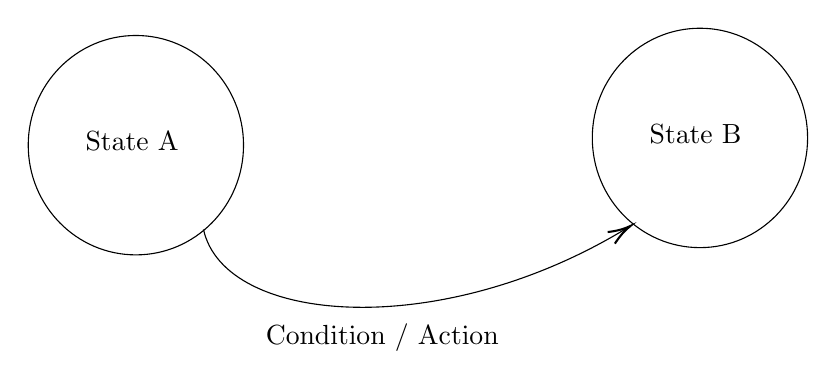
\begin{tikzpicture}[x=0.75pt,y=0.75pt,yscale=-1,xscale=1]
%uncomment if require: \path (0,777); %set diagram left start at 0, and has height of 777

%Shape: Ellipse [id:dp7032860404022366]
\draw   (10,63.35) .. controls (10,34.16) and (33.22,10.49) .. (61.87,10.49) .. controls (90.51,10.49) and (113.73,34.16) .. (113.73,63.35) .. controls (113.73,92.54) and (90.51,116.2) .. (61.87,116.2) .. controls (33.22,116.2) and (10,92.54) .. (10,63.35) -- cycle ;
%Shape: Ellipse [id:dp2228367254212833]
\draw   (281.77,59.85) .. controls (281.77,30.66) and (304.99,7) .. (333.63,7) .. controls (362.28,7) and (385.5,30.66) .. (385.5,59.85) .. controls (385.5,89.05) and (362.28,112.71) .. (333.63,112.71) .. controls (304.99,112.71) and (281.77,89.05) .. (281.77,59.85) -- cycle ;
%Curve Lines [id:da7146299088305332]
\draw    (94.44,103.97) .. controls (104.68,150.04) and (209.13,158.06) .. (298.85,103.06) ;
\draw [shift={(300.2,102.23)}, rotate = 508.15] [color={rgb, 255:red, 0; green, 0; blue, 0 }  ][line width=0.75]    (10.93,-3.29) .. controls (6.95,-1.4) and (3.31,-0.3) .. (0,0) .. controls (3.31,0.3) and (6.95,1.4) .. (10.93,3.29)   ;

% Text Node
\draw (36.37,55.72) node [anchor=north west][inner sep=0.75pt]   [align=left] {State A};
% Text Node
\draw (308.13,52.23) node [anchor=north west][inner sep=0.75pt]   [align=left] {State B};
% Text Node
\draw (123.18,148.33) node [anchor=north west][inner sep=0.75pt]   [align=left] {Condition / Action};
\end{tikzpicture}

}
\end{center}

\vspace{0.5cm}

\begin{minipage}[t]{0.6\textwidth}
États: représentés par des cercles

- État initial (triangle/flèche isolée)

- États intermédiaires

- État final (double cercle)\\
\end{minipage}
\begin{minipage}[t]{0.8\textwidth}
Transitions: représentées par des flèches

- D'un état à un autre

- D'un état à lui-même (récursif)

- Transition lambda/epsilon (vide)\\
\end{minipage}

\begin{center}
\resizebox{0.6\textwidth}{!}{
    \tikzset{every picture/.style={line width=0.75pt}} %set default line width to 0.75pt

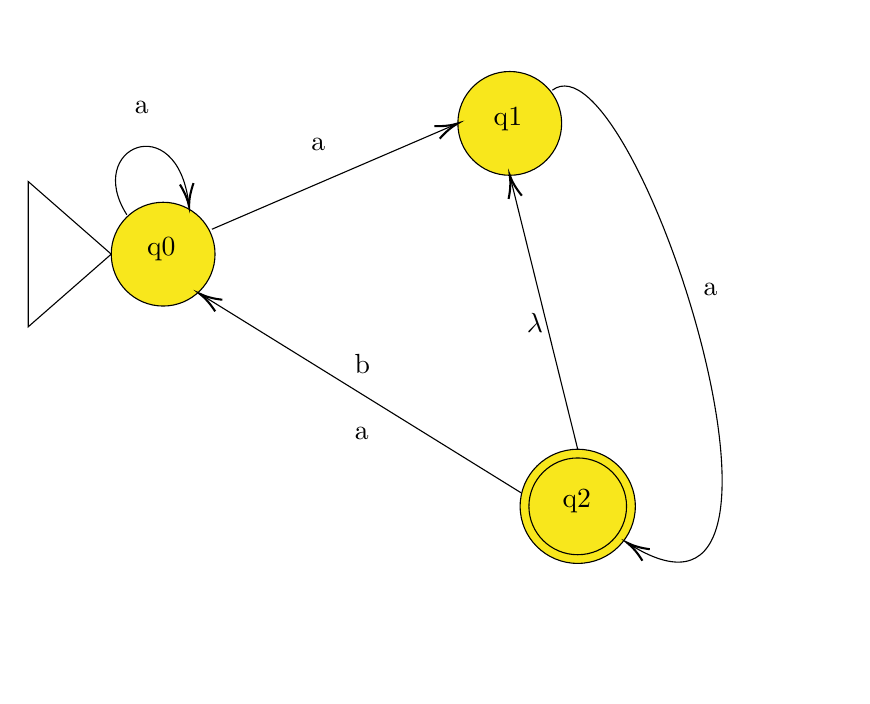
\begin{tikzpicture}[x=0.75pt,y=0.75pt,yscale=-1,xscale=1]
%uncomment if require: \path (0,777); %set diagram left start at 0, and has height of 777

%Flowchart: Extract [id:dp2213490168388459]
\draw   (48,96) -- (8,131) -- (8,61) -- cycle ;
%Shape: Circle [id:dp9156481012483882]
\draw  [fill={rgb, 255:red, 248; green, 231; blue, 28 }  ,fill opacity=1 ] (48,96) .. controls (48,82.19) and (59.19,71) .. (73,71) .. controls (86.81,71) and (98,82.19) .. (98,96) .. controls (98,109.81) and (86.81,121) .. (73,121) .. controls (59.19,121) and (48,109.81) .. (48,96) -- cycle ;
%Shape: Circle [id:dp8937236461295127]
\draw  [fill={rgb, 255:red, 248; green, 231; blue, 28 }  ,fill opacity=1 ] (215,33) .. controls (215,19.19) and (226.19,8) .. (240,8) .. controls (253.81,8) and (265,19.19) .. (265,33) .. controls (265,46.81) and (253.81,58) .. (240,58) .. controls (226.19,58) and (215,46.81) .. (215,33) -- cycle ;
%Shape: Ellipse [id:dp6295802993903136]
\draw  [fill={rgb, 255:red, 248; green, 231; blue, 28 }  ,fill opacity=1 ] (245,217.5) .. controls (245,202.31) and (257.42,190) .. (272.75,190) .. controls (288.08,190) and (300.5,202.31) .. (300.5,217.5) .. controls (300.5,232.69) and (288.08,245) .. (272.75,245) .. controls (257.42,245) and (245,232.69) .. (245,217.5) -- cycle ;
%Shape: Ellipse [id:dp23912526643664667]
\draw  [fill={rgb, 255:red, 248; green, 231; blue, 28 }  ,fill opacity=1 ] (249.23,217.5) .. controls (249.23,204.63) and (259.76,194.19) .. (272.75,194.19) .. controls (285.74,194.19) and (296.27,204.63) .. (296.27,217.5) .. controls (296.27,230.37) and (285.74,240.81) .. (272.75,240.81) .. controls (259.76,240.81) and (249.23,230.37) .. (249.23,217.5) -- cycle ;
%Straight Lines [id:da07722341343778594]
\draw    (245.5,211) -- (92.2,116.05) ;
\draw [shift={(90.5,115)}, rotate = 391.77] [color={rgb, 255:red, 0; green, 0; blue, 0 }  ][line width=0.75]    (10.93,-3.29) .. controls (6.95,-1.4) and (3.31,-0.3) .. (0,0) .. controls (3.31,0.3) and (6.95,1.4) .. (10.93,3.29)   ;
%Straight Lines [id:da5881939013667715]
\draw    (96.5,84) -- (213.16,33.79) ;
\draw [shift={(215,33)}, rotate = 516.71] [color={rgb, 255:red, 0; green, 0; blue, 0 }  ][line width=0.75]    (10.93,-3.29) .. controls (6.95,-1.4) and (3.31,-0.3) .. (0,0) .. controls (3.31,0.3) and (6.95,1.4) .. (10.93,3.29)   ;
%Curve Lines [id:da24978032388245308]
\draw    (260.5,17) .. controls (300.3,-12.85) and (399.5,298.86) .. (298.04,235.98) ;
\draw [shift={(296.5,235)}, rotate = 392.78999999999996] [color={rgb, 255:red, 0; green, 0; blue, 0 }  ][line width=0.75]    (10.93,-3.29) .. controls (6.95,-1.4) and (3.31,-0.3) .. (0,0) .. controls (3.31,0.3) and (6.95,1.4) .. (10.93,3.29)   ;
%Straight Lines [id:da3348378214953378]
\draw    (272.75,190) -- (240.48,59.94) ;
\draw [shift={(240,58)}, rotate = 436.07] [color={rgb, 255:red, 0; green, 0; blue, 0 }  ][line width=0.75]    (10.93,-3.29) .. controls (6.95,-1.4) and (3.31,-0.3) .. (0,0) .. controls (3.31,0.3) and (6.95,1.4) .. (10.93,3.29)   ;
%Curve Lines [id:da1693586185231678]
\draw    (55.5,77) .. controls (34.71,44.33) and (79.59,25.38) .. (85.34,71.58) ;
\draw [shift={(85.5,73)}, rotate = 264.05] [color={rgb, 255:red, 0; green, 0; blue, 0 }  ][line width=0.75]    (10.93,-3.29) .. controls (6.95,-1.4) and (3.31,-0.3) .. (0,0) .. controls (3.31,0.3) and (6.95,1.4) .. (10.93,3.29)   ;

% Text Node
\draw (247,123) node [anchor=north west][inner sep=0.75pt]   [align=left] {$\lambda$};
% Text Node
\draw (64,87) node [anchor=north west][inner sep=0.75pt]   [align=left] {q0};
% Text Node
\draw (231,24) node [anchor=north west][inner sep=0.75pt]   [align=left] {q1};
% Text Node
\draw (264.19,208.07) node [anchor=north west][inner sep=0.75pt]   [align=left] {q2};
% Text Node
\draw (58,21) node [anchor=north west][inner sep=0.75pt]   [align=left] {a};
% Text Node
\draw (332,109) node [anchor=north west][inner sep=0.75pt]   [align=left] {a};
% Text Node
\draw (143,39) node [anchor=north west][inner sep=0.75pt]   [align=left] {a};
% Text Node
\draw (164,143) node [anchor=north west][inner sep=0.75pt]   [align=left] {b\\ \\a};
\end{tikzpicture}

}
\end{center}

\textbf{Déterministe vs non-déterministe}

Après avoir reconnu "abb", sommes-nous à l'état final ou bien toujours à l'état initial? Impossible à dire avec certitude.

\begin{center}
\resizebox{\textwidth}{!}{
    \tikzset{every picture/.style={line width=0.75pt}} %set default line width to 0.75pt

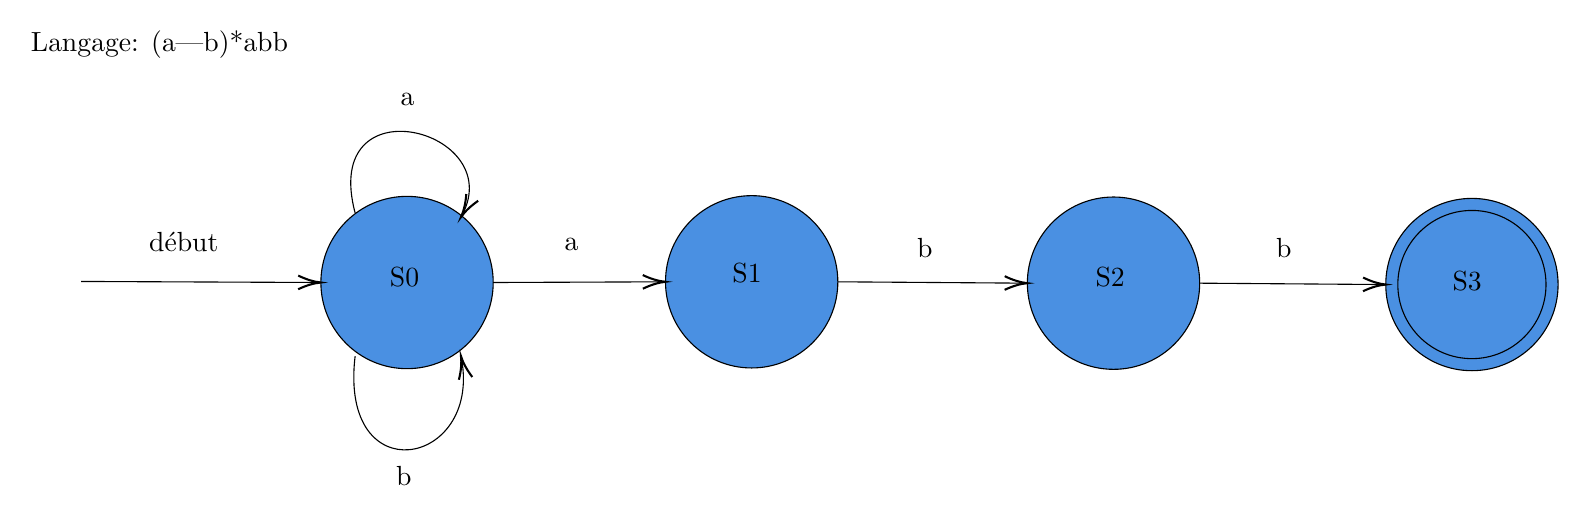
\begin{tikzpicture}[x=0.75pt,y=0.75pt,yscale=-1,xscale=1]
%uncomment if require: \path (0,777); %set diagram left start at 0, and has height of 777

%Shape: Circle [id:dp9851709242772706]
\draw  [fill={rgb, 255:red, 74; green, 144; blue, 226 }  ,fill opacity=1 ] (161,135.51) .. controls (161,112.58) and (179.58,94) .. (202.51,94) .. controls (225.43,94) and (244.02,112.58) .. (244.02,135.51) .. controls (244.02,158.43) and (225.43,177.02) .. (202.51,177.02) .. controls (179.58,177.02) and (161,158.43) .. (161,135.51) -- cycle ;
%Shape: Circle [id:dp2634550867663098]
\draw  [fill={rgb, 255:red, 74; green, 144; blue, 226 }  ,fill opacity=1 ] (327.04,135.17) .. controls (327.04,112.24) and (345.62,93.66) .. (368.55,93.66) .. controls (391.47,93.66) and (410.06,112.24) .. (410.06,135.17) .. controls (410.06,158.09) and (391.47,176.68) .. (368.55,176.68) .. controls (345.62,176.68) and (327.04,158.09) .. (327.04,135.17) -- cycle ;
%Shape: Circle [id:dp7244233597696788]
\draw  [fill={rgb, 255:red, 74; green, 144; blue, 226 }  ,fill opacity=1 ] (501.38,135.83) .. controls (501.38,112.91) and (519.96,94.32) .. (542.89,94.32) .. controls (565.81,94.32) and (584.4,112.91) .. (584.4,135.83) .. controls (584.4,158.76) and (565.81,177.34) .. (542.89,177.34) .. controls (519.96,177.34) and (501.38,158.76) .. (501.38,135.83) -- cycle ;
%Shape: Circle [id:dp07451760427696097]
\draw  [fill={rgb, 255:red, 74; green, 144; blue, 226 }  ,fill opacity=1 ] (674.06,136.49) .. controls (674.06,113.57) and (692.64,94.98) .. (715.57,94.98) .. controls (738.49,94.98) and (757.08,113.57) .. (757.08,136.49) .. controls (757.08,159.42) and (738.49,178) .. (715.57,178) .. controls (692.64,178) and (674.06,159.42) .. (674.06,136.49) -- cycle ;
%Shape: Ellipse [id:dp8941531755272224]
\draw  [fill={rgb, 255:red, 74; green, 144; blue, 226 }  ,fill opacity=1 ] (679.87,136.49) .. controls (679.87,116.78) and (695.85,100.79) .. (715.57,100.79) .. controls (735.28,100.79) and (751.26,116.78) .. (751.26,136.49) .. controls (751.26,156.21) and (735.28,172.19) .. (715.57,172.19) .. controls (695.85,172.19) and (679.87,156.21) .. (679.87,136.49) -- cycle ;
%Straight Lines [id:da9727164886338506]
\draw    (45.5,135) -- (159,135.5) ;
\draw [shift={(161,135.51)}, rotate = 180.25] [color={rgb, 255:red, 0; green, 0; blue, 0 }  ][line width=0.75]    (10.93,-3.29) .. controls (6.95,-1.4) and (3.31,-0.3) .. (0,0) .. controls (3.31,0.3) and (6.95,1.4) .. (10.93,3.29)   ;
%Straight Lines [id:da38657510871619216]
\draw    (244.02,135.51) -- (325.04,135.18) ;
\draw [shift={(327.04,135.17)}, rotate = 539.77] [color={rgb, 255:red, 0; green, 0; blue, 0 }  ][line width=0.75]    (10.93,-3.29) .. controls (6.95,-1.4) and (3.31,-0.3) .. (0,0) .. controls (3.31,0.3) and (6.95,1.4) .. (10.93,3.29)   ;
%Straight Lines [id:da45803946933994955]
\draw    (410.06,135.17) -- (499.38,135.82) ;
\draw [shift={(501.38,135.83)}, rotate = 180.41] [color={rgb, 255:red, 0; green, 0; blue, 0 }  ][line width=0.75]    (10.93,-3.29) .. controls (6.95,-1.4) and (3.31,-0.3) .. (0,0) .. controls (3.31,0.3) and (6.95,1.4) .. (10.93,3.29)   ;
%Straight Lines [id:da19707808507116387]
\draw    (584.4,135.83) -- (672.06,136.48) ;
\draw [shift={(674.06,136.49)}, rotate = 180.42] [color={rgb, 255:red, 0; green, 0; blue, 0 }  ][line width=0.75]    (10.93,-3.29) .. controls (6.95,-1.4) and (3.31,-0.3) .. (0,0) .. controls (3.31,0.3) and (6.95,1.4) .. (10.93,3.29)   ;
%Curve Lines [id:da7298553041692105]
\draw    (177.5,102) .. controls (160.67,38.64) and (250.67,61.53) .. (229.19,102.75) ;
\draw [shift={(228.5,104)}, rotate = 299.74] [color={rgb, 255:red, 0; green, 0; blue, 0 }  ][line width=0.75]    (10.93,-3.29) .. controls (6.95,-1.4) and (3.31,-0.3) .. (0,0) .. controls (3.31,0.3) and (6.95,1.4) .. (10.93,3.29)   ;
%Curve Lines [id:da9993413766624407]
\draw    (177.5,171) .. controls (169.58,237.33) and (238.11,224.27) .. (228.81,172.58) ;
\draw [shift={(228.5,171)}, rotate = 438.27] [color={rgb, 255:red, 0; green, 0; blue, 0 }  ][line width=0.75]    (10.93,-3.29) .. controls (6.95,-1.4) and (3.31,-0.3) .. (0,0) .. controls (3.31,0.3) and (6.95,1.4) .. (10.93,3.29)   ;

% Text Node
\draw (198,43) node [anchor=north west][inner sep=0.75pt]   [align=left] {a};
% Text Node
\draw (277,113) node [anchor=north west][inner sep=0.75pt]   [align=left] {a};
% Text Node
\draw (447,113) node [anchor=north west][inner sep=0.75pt]   [align=left] {b};
% Text Node
\draw (620,113) node [anchor=north west][inner sep=0.75pt]   [align=left] {b};
% Text Node
\draw (196,223) node [anchor=north west][inner sep=0.75pt]   [align=left] {b};
% Text Node
\draw (20,13) node [anchor=north west][inner sep=0.75pt]   [align=left] {Langage: (a|b)*abb};
% Text Node
\draw (77,110) node [anchor=north west][inner sep=0.75pt]   [align=left] {début};
% Text Node
\draw (193,127) node [anchor=north west][inner sep=0.75pt]   [align=left] {S0};
% Text Node
\draw (358,125) node [anchor=north west][inner sep=0.75pt]   [align=left] {S1};
% Text Node
\draw (533,127) node [anchor=north west][inner sep=0.75pt]   [align=left] {S2};
% Text Node
\draw (705,129) node [anchor=north west][inner sep=0.75pt]   [align=left] {S3};

\end{tikzpicture}

}
\end{center}

\newpage

\subsection{Équivalences}

On a décrit trois manières d'exprimer la même chose: les langages rationnels/réguliers/reconnaissables.

\begin{center}
\resizebox{0.6\textwidth}{!}{
    \tikzset{every picture/.style={line width=0.75pt}} %set default line width to 0.75pt

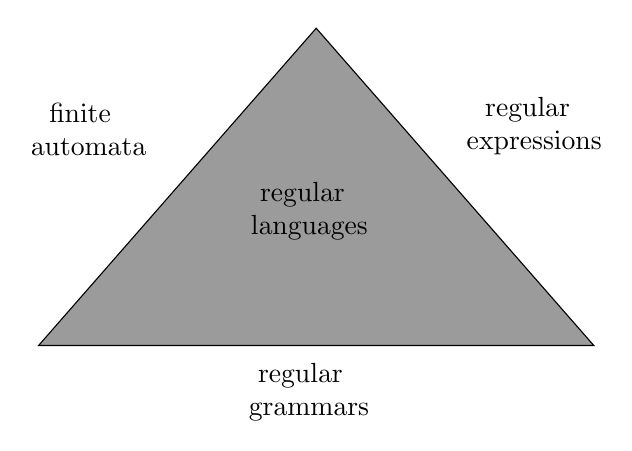
\begin{tikzpicture}[x=0.75pt,y=0.75pt,yscale=-1,xscale=1]
%uncomment if require: \path (0,777); %set diagram left start at 0, and has height of 777

%Shape: Triangle [id:dp3679553887605198]
\draw  [fill={rgb, 255:red, 155; green, 155; blue, 155 }  ,fill opacity=1 ] (152.75,10) -- (286.5,162.86) -- (19,162.86) -- cycle ;

% Text Node
\draw (120,83) node [anchor=north west][inner sep=0.75pt]   [align=left] { \ regular\\languages};
% Text Node
\draw (14,45) node [anchor=north west][inner sep=0.75pt]   [align=left] { \ \ finite\\automata};
% Text Node
\draw (224,42) node [anchor=north west][inner sep=0.75pt]   [align=left] { \ \ regular\\expressions};
% Text Node
\draw (119,170) node [anchor=north west][inner sep=0.75pt]   [align=left] { \ regular\\grammars};
\end{tikzpicture}

}
\end{center}

\subsection{Morphologie}

La morphologie permet soit de gérer des variantes de mots (morphologie flexionelle) soit de construire des nouveaux mots. \\

Au niveau de la construction, on peut soit faire une dérivation ("affixation", en conservant ou changeant la catégorie du mot) soit faire de la composition (noms composés, adjectifs composés, verbes composés, adverbes composés). \\

\subsection{Transducteurs}

FST: Finite-state transducers.\\

Similaires aux FSA mais la condition pour passer d'un état à un autre est remplacée par une action à effectuer. Utilisés soit pour analyser une chaine existante, soit pour générer une chaîne à partir de traits.\\

\subsection{Stemming}

\textbf{Racinisation (stemming)}

Version simplifiée de l'analyse morphologique. Ne s'encombre pas du lexique: principalement basée sur la désuffixation (vs lemmatisation). Moins précise mais beaucoup plus rapide. Très utilisée par les moteurs de recherche.\\

\textbf{Porter stemmer}

Crée par Martin Porter (1980). Ensemble de règles simples en cascade, par exemple:

\begin{itemize}
    \item SSES $\rightarrow$ SS
    \item ING $\rightarrow$ epsilon
    \item ATIONAL $\rightarrow$ ATE\\
\end{itemize}

Mais, ce n'est pas hyper précis, il y a de nombreux problèmes, comme par exemple:

\begin{itemize}
    \item organization $\rightarrow$ organ (sens perdu)
    \item policy $\rightarrow$ police (sens perdu)
    \item Adobe Illustrator $\rightarrow$ illustrate (nom propre a un sens particulier)\\
\end{itemize}

\subsection{Segmentation (tokenization)}

Séparation d'un texte en phrases et des phrases en mots. Étape cruciale pour le succès des stades suivants (analyse morphologique, traduction automatique, etc).\\

\textbf{Séparation en phrases}

Approche naïve: séparation par un point suivi d'un espace. Mais malheureusement cela ne couvre absolument pas tous les cas.\\

\textbf{Parts of Speech}

Les petites poules du couvent les couvent bien \\

\begin{minipage}[t]{0.5\textwidth}
\begin{itemize}
\item Les: DET
\item petites: ADJ
\item poules: NOM
\item du: PREP
\end{itemize}
\end{minipage}
\begin{minipage}[t]{0.5\textwidth}
\begin{itemize}
 \item couvent: NOM
\item les: PRON
\item couvent: VB
\item bien: ADV
\end{itemize}
\end{minipage}

\subsection{Tagging}

\textbf{Tagsets}

Listes des "parties du discours" (catégories)\\

Granularités très variables:
\begin{itemize}
    \item French Treebank: 15 catégories grammaticales
    \item Penn Treebank: 36 (45 avec la ponctuation)
    \item C5: 67
    \item Brown: 87
    \item Sinica (chinois): 294!\\
\end{itemize}

\textbf{PoS tagging}

Étiquetage morpho-syntaxique/grammatical.

Trois approches principales:
\begin{itemize}
    \item linguistiques (règles)
    \item statistique (HMM - hidden markov models, Viterbi)
    \item transformative (Brill tagger)\\
\end{itemize}

\textbf{Taggers linguistiques}

Choix parmi les différents candidats trouvés dans un dictionnaire. Basés sur une succession de règles très complexes. Exemple pour l'anglais: ENGTWOL.\\

\textbf{HMM taggers}

Approche probabiliste basée sur le modèle bayésien d'inférence (Hidden Markov Model - 1763). Choix de la séquence de tags la plus probable parmi toutes les séquences possibles, en fonction des mots observés.

Prémisses simplificatrices: la probabilité d'un mot ne dépend pas du contexte (faux, mais c'est pour simplifier); la probabilité d'un tag ne dépend que du précédent (modèle des bigrammes)

Approximation = produit entre: la probabilité d'un mot hors contexte (fréquence) pour un tag donné; la probabilité de transition d'un tag à un autre\\

\textbf{Brill tagger}

Approche hybride basée sur des règles ET un entrainement statistique (machine learning). Technique supervisée: nécessite un corpus annoté manuellement pour l'apprentissage. Première approximation probabiliste puis règles de transformation.

\newpage
\lecture{7}{mercredi 18 mars 2020}
\vspace{-1.2cm}

\section{Aspects syntaxiques}

\textbf{Syntaxe}: Du grec ancien \textgreek{σύνταξις} (súntaxis) qui signifie "arrangement" ou "mise en ordre". Façon dont les mots se combinent pour former des phrases structurées. Unité syntaxique = syntagme (groupe de mots).\\

\textbf{Structure en arbre}

\begin{center}
\resizebox{0.6\textwidth}{!}{
    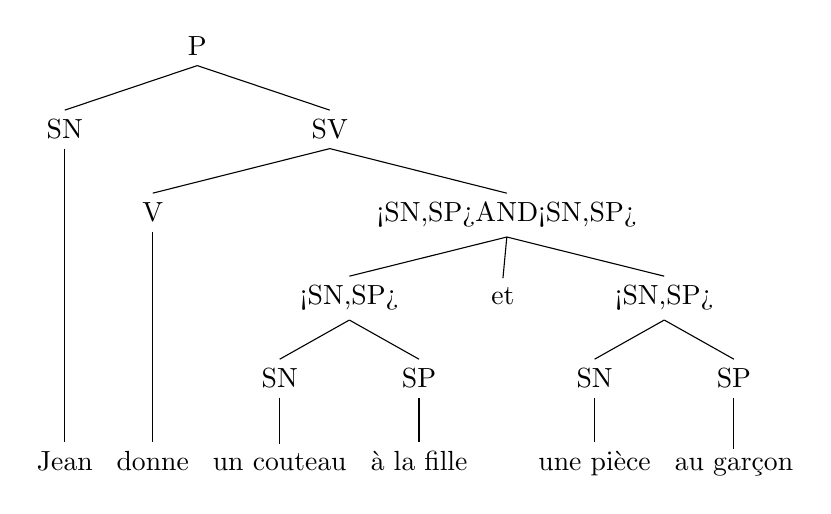
\begin{tikzpicture}
\tikzset{frontier/.style={distance from root=150pt}}

\Tree [.P
    [.SN Jean ]
    [.SV
        [.V donne ] [.<SN,SP>AND<SN,SP>
            [.<SN,SP>
                [.SN {un couteau} ] [.SP {à la fille} ]
            ]
            [.et ]
            [.<SN,SP>
                [.SN {une pièce} ] [.SP {au garçon} ]
            ]
        ]
    ]
]

\end{tikzpicture}

}
\end{center}

\textbf{Structure plate (crochets)}

[P [SN Jean ] [SV [V donne ] [<SN,SP>AND<SN,SP> [<SN,SP> [SN un couteau ] [SP à la fille ] ] [et ] [<SN,SP> [SN une pièce ] [SP au garçon ] ] ] ] ] \\

\textbf{Constituants}

P (S) phrase (symbole de départ)

SN (NP) syntagme nominal

SV (VP) syntagme verbal

SP (PP) syntagme prépositionnel

N nom

V verbe

Prep préposition\\

\textbf{Grammaire context-free (CFG)}

Simplification du langage naturel mais plus flexible qu'une grammaire régulière. Permet de modéliser les relations entre constituants. Ensemble de règles pour organiser symboles grammaticaux et unités lexicales. Génération et analyse (parsing).\\

Exemple:

S $\rightarrow$ NP VP

NP $\rightarrow$ 'the man' | 'the book'

VP $\rightarrow$ Verb NP

(VP $\rightarrow$ Verb)

Verb $\rightarrow$ 'took' | 'read' \\


\textbf{Grammaire générative}

Un sous-langage est défini par l'ensemble des phrases générées par la grammaire. Puissance générative : une infinité de phrases peut être générée par un ensemble fini de règles. Équilibre à trouver entre sous-génération (silence) et sur-génération (bruit). \\

\textbf{Treebanks}

Corpus de textes annotés avec leurs structures syntaxiques correspondantes. Une révolution pour la TAL! \\

Exemples: Penn Treebank (1992) et French Treebank (1997)\\

(SENT (NP-SUJ (D La) (N diminution)) (VN (V
paraît)) (PONCT ,) (ADV toutefois) (PONCT ,) (AP-
ATS (ADV moins) (A nette)) (PP-MOD (P en) (NP
(N France)) (COORD (C et) (PP (P en) (NP (N
Italie))))) (PONCT .)) \\

\textbf{Parsing (analyse grammaticale)}

Tâche qui consiste à reconnaître une phrase et à y assigner une structure syntaxique.

Applications diverses: correction grammaticale, TA, question answering.

Recherche de l'arbre correct parmi l'ensemble des arbres possibles (cf. treebanks).\\

\textbf{Stratégies de recherche}

"Marie voit un chat."\\

Deux contraintes:

\begin{itemize}
    \item grammaticale : former une phrase (symbole P)
    \item lexicale : utiliser les quatre mots dans l'ordre
\end{itemize}

Deux approches:

\begin{itemize}
    \item top-down : en partant de l'objectif à atteindre
    \item bottom-up : en partant des données à utiliser\\
\end{itemize}

\textbf{Top-down}

On part du symbole de départ P

Règles de réécriture gauche $\rightarrow$ droite

L'analyse réussit si le symbole P couvre une structure qui contient tous les mots de la phrase dans le bon ordre.\\

\textbf{Bottom-up}

On part des mots de la phrase

Règles de réécriture gauche $\leftarrow$ droite

L'analyse réussit si le parser parvient à atteindre le symbole P.\\


\textbf{Exploration de l'espace de recherche}

Depth-first : d'abord les nouvelles options (en série).

Breadth-first : d'abord les options existantes (en parallèle).

Même résultat mais chemins différents pour y parvenir.\\

\textbf{Chart parsing}

Basé sur la programmation dynamique

Évite de répéter plusieurs fois une analyse en conservant les sous-arbres en mémoire

Résout partiellement le problème de l'ambiguïté en stockant des arbres parallèles\\

\textbf{Shallow parsing}

Une analyse syntaxique complète peut être assez lourde et prendre un certain temps en raison du nombre d'arbres à générer.

Alternative : analyse partielle en surface

Suffisant pour beaucoup d'applications\\

\textbf{Chunking}

Méthode fréquente de shallow parsing

Identification et classification de constituants dans une structure plate et non-imbriquée

Pas de validation jusqu'au niveau de la phrase

Complexité variable en fonction des besoins\\

\textbf{Structures de traits (features)}

Permettent d'encoder des informations (genre, nombre, personne, temps, mode…) de manière plus flexible qu'avec une grammaire CFG.

"Context-sensitive grammars".\\

\newpage
\lecture{8}{mercredi 25 mars 2020}
\vspace{-1.2cm}

\section{Aspects sémantiques}


Exercices

« Le Gauguin est un bar » : Bar(Gauguin)

« Le Snack 44 sert des sandwiches » : Servir(Snack 44, Sandwiches)

« Je veux manger en terrasse, ou alors pas cher » : Vouloir(Locuteur, x) AND Restaurant(x) AND ( Avoir(x, Terrasse) OR NOT Etre(x, Cher) )

« J'aime les restos italiens et japonais » : Restaurant(x, Italien) OU Restaurant(x, Japonais)

« Peut-on trouver un restaurant végétarien à Ixelles ? » : Exists x: Restaurant(x) AND Type(x, Vegetarien) AND CodePostal(x, 1050)

« Les cafés du Cimetière sont proches de l'ULB » : Pourtout x Cafe(x) : Proche(x, Cimetiered'Ixelles) -> Distance(x, ULB) < 5km


\end{document}
